%Este trabalho está licenciado sob a Licença Creative Commons Atribuição-CompartilhaIgual 3.0 Não Adaptada. Para ver uma cópia desta licença, visite https://creativecommons.org/licenses/by-sa/3.0/ ou envie uma carta para Creative Commons, PO Box 1866, Mountain View, CA 94042, USA.

\documentclass[../livro.tex]{subfiles}  %%DM%%Escolher document class and options article, etc

%define o diretório principal
\providecommand{\dir}{..}

%%%%%%%%%%%%%%%%%%%%%%%%%%%%%%%%%%%%%%%%%%%%%
%%%%%%%%%%%%INICIO DO DOCUMENTO%%%%%%%%%%%%%%
%%%%%%%%%%%%%%%%%%%%%%%%%%%%%%%%%%%%%%%%%%%%%

\begin{document}

\chapter{Semana 11}


Nesta semana, nós começamos uma abordagem um pouco mais geométrica de espaços vetoriais: ângulo entre vetores, comprimento de vetores, ortogonalidade. Estes conceitos já são de nossa familiaridade da geometria euclideana (em $\mathbb{R}^2$ e $\mathbb{R}^3$). No entanto, é também nosso objetivo estender estes conceitos para dimensões maiores do que $3$.


\section{Comprimento, ângulos e o produto escalar}

Se, na base canônica (isto é, no sistema de coordenadas usual) do espaço $\mathbb{R}^3$, representamos um vetor por
\begin{equation}
\vec{v} =
\begin{bmatrix}
v_1 \\ v_2 \\ v_3
\end{bmatrix},
\end{equation} então o seu \textbf{comprimento} (ou \textbf{magnitude} ou \textbf{norma}) é dado por
\begin{equation}
\|\vec{v}\| = \sqrt{v_1^2 + v_2^2 + v_3^2}.
\end{equation} Esta é uma instância do Teorema de Pitágoras\footnote{Duas aplicações do Teorema de Pitágoras usual do plano. Uma para obter o comprimento $\sqrt{v_1^2 + v_2^2}$ da diagonal que está no plano $xy$ e a outra para obter $\|\vec{v}\|$.}.

\begin{figure}[h!]
	\begin{center}
		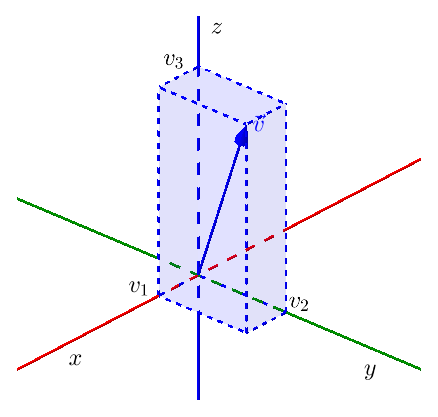
\includegraphics[width=0.3\linewidth]{\dir/Semana11/semana11-coord}
	\end{center}
\end{figure}

\noindent A definição acima pode ser generalizada para dimensão $n$ qualquer:
\begin{equation}
\vec{v} =
\begin{bmatrix}
v_1 \\ v_2 \\ \vdots \\ v_n
\end{bmatrix} \quad \rightsquigarrow \quad \|\vec{v}\| = \sqrt{v_1^2 + v_2^2 + \cdots + v_n^2}.
\end{equation}


O \textbf{produto escalar} ou \textbf{produto interno} entre dois vetores $\vec{v}$ e $\vec{w}$ é um número (também dito escalar) associado com estes dois vetores. Em coordenadas, se $\vec{v} = (v_1, v_2, v_3)$ e $\vec{w} = (w_1, w_2, w_3)$ são vetores do espaço tridimensional $\mathbb{R}^3$, temos
\begin{equation}
\vec{v} \cdot \vec{w} = v_1 w_1 + v_2 w_2 + v_3 w_3.
\end{equation} Vejamos que realmente o produto escalar tem a ver com o ângulo entre dois vetores. Isto é uma consequência da Lei dos Cossenos, que nos diz que
\begin{equation}
\|\vec{v} - \vec{w}\|^2 = \|\vec{v}\|^2 + \|\vec{w}\|^2 - 2 \|\vec{v}\| \|\vec{w}\| \cos \theta,
\end{equation} onde $\theta$ é o ângulo entre $\vec{v}$ e $\vec{w}$. 

	\begin{center}
		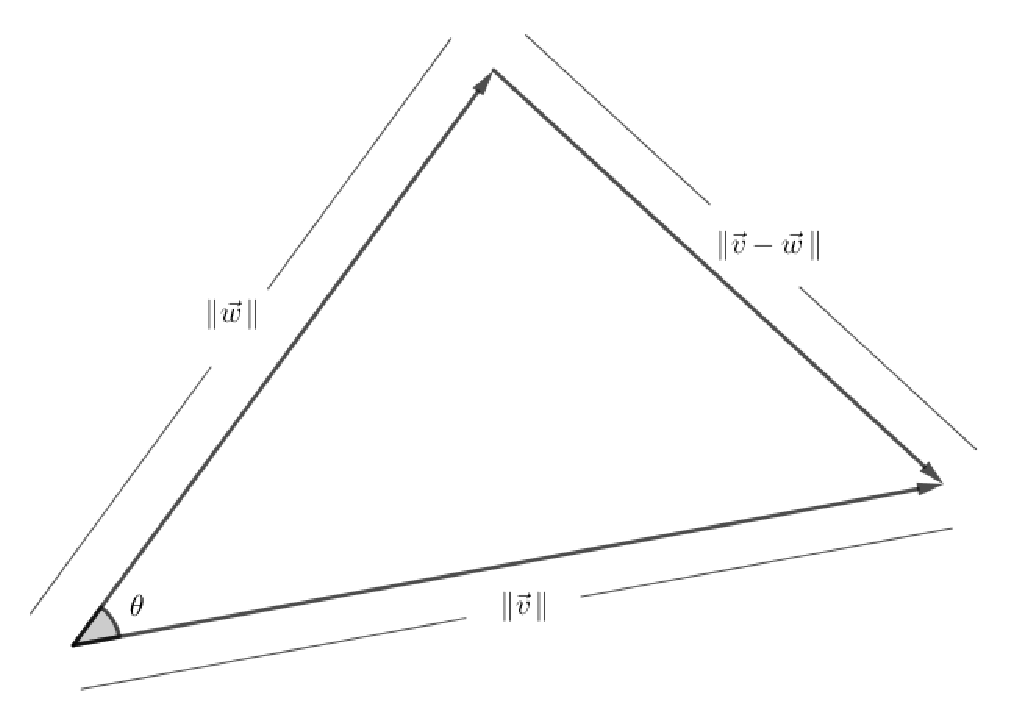
\includegraphics[width=0.7\linewidth]{\dir/Semana11/semana11-cossenos}
	\end{center}

\noindent Escrevendo estes comprimentos em termos das coordenadas e fazendo os cancelamentos necessários, chegamos na seguinte identidade:
\begin{equation}
v_1 w_1 + v_2 w_2 + v_3 w_3 = \|\vec{v}\| \|\vec{w}\| \cos \theta, \quad \text{ isto é,} \quad \vec{v} \cdot \vec{w} = \|\vec{v}\| \|\vec{w}\| \cos \theta.
\end{equation}


Motivados pelos conceitos acima, consideramos
\begin{equation}
\vec{x} =
\begin{bmatrix}
x_1 \\ x_2 \\ \vdots \\ x_n
\end{bmatrix} \quad \text{e} \quad \vec{y} =
\begin{bmatrix}
y_1 \\ y_2 \\ \vdots \\ y_n
\end{bmatrix}
\end{equation} vetores de $\mathbb{R}^n$ representados na base canônica, e definimos o \textbf{produto escalar} ou \textbf{produto interno} entre $\vec{x}$ e $\vec{y}$:
\begin{equation}
\vec{x} \cdot \vec{y} = x_1 y_1 + x_2 y_2 + \cdots + x_n y_n.
\end{equation} O ângulo entre $\vec{x}$ e $\vec{y}$, para $n$ qualquer, pode então ser \textit{definido} pela equação
\begin{equation}
\cos \theta = \frac{\vec{x} \cdot \vec{y}}{\|\vec{x}\| \|\vec{y}\|}.
\end{equation} Embora abstratos, estes conceitos são bem fundamentados geometricamente. Dois vetores (linearmente independentes) de um espaço vetorial $n$-dimensional geram um subespaço vetorial de dimensão $2$. Este pode, por sua vez, pode ser pensado como um plano que passa pela origem de $\mathbb{R}^n$. Assim, podemos imaginar o ângulo entre estes vetores naturalmente.

\begin{proposition}[Principais propriedades do produto escalar]
	Para $\vec{x}, \vec{y}, \vec{z} \in \mathbb{R}^n$ e $c \in \mathbb{R}$ um escalar, temos as seguintes propriedades
	\begin{enumerate}
		\item  $\vec{x} \cdot \vec{y} = \vec{y} \cdot \vec{x}$
		\item  $(\vec{x} + \vec{y}) \cdot \vec{z} = \vec{x} \cdot \vec{z} + \vec{y} \cdot \vec{z}$
		\item  $(c\vec{x}) \cdot \vec{y} = c \vec{x} \cdot \vec{y} = \vec{x} \cdot (c\vec{y})$
		\item  $\vec{x} \cdot \vec{x} \ge 0$ e $\, \vec{x} \cdot \vec{x} = 0$ se, e somente se, $\vec{x} = \vec{0}$;
		\item  $\|\vec{x}\| = \sqrt{\vec{x} \cdot \vec{x}}$;
		\item  $\| c \vec{x} \| =  |c| \| \vec{x} \|$.
	\end{enumerate}
\end{proposition}

Estas propriedades são todas de fácil verificação (e são deixadas para o leitor verificar, como exercício).

\begin{example}
	Considere os vetores de $\mathbb{R}^5$ escritos na base canônica:
	\begin{equation}
	\vec{x} =
	\begin{bmatrix}
	-1 \\ 2 \\ 0 \\ 3 \\ -1
	\end{bmatrix} \quad \text{e} \quad \vec{y} =
	\begin{bmatrix}
	4 \\ 3 \\ -1 \\ -11 \\ 1
	\end{bmatrix}
	\end{equation} Assim, temos
	\begin{equation}
	\vec{x} \cdot \vec{y} = (-1)\cdot 4 + 2 \cdot 3 + 0 \cdot (-1) +3 \cdot(-11) + (-1)\cdot 1 = -4 + 6 +0 -33 -1 = -31.
	\end{equation} Da mesma forma, podemos calcular os comprimentos
	\begin{equation}
	\| \vec{x} \| = \sqrt{(-1)^2 + 2^2 + 0^2 + 3^2 + (-1)^2} = \sqrt{15} \quad \text{e} \quad \| \vec{y} \| = \sqrt{4^2 + 3^2 + (-1)^2 + (-11)^2 + 1^2} = \sqrt{148}.
	\end{equation} Logo, o ângulo $\theta$ entre estes vetores satisfaz (utilizamos uma calculadora para calcular as raízes quadradas e a função inversa do cosseno):
	\begin{equation}
	\cos \theta = \frac{\vec{x} \cdot \vec{y}}{\|\vec{x}\| \|\vec{y}\|} = \frac{-31}{\sqrt{15} \, \sqrt{148}} \simeq -0,65794 \implies  \theta \simeq 2,28887634 \textrm{ radianos} \simeq 131,12^{\text{o}}. \ \lhd
	\end{equation}
\end{example}

\begin{example}
	Considere um vetor tridimensional
	\begin{equation}
	\vec{u} =
	\begin{bmatrix}
	2 \\ 3 \\ -1
	\end{bmatrix}.
	\end{equation} Já sabemos a multiplicação de um escalar pelo vetor $\vec{u}$ muda o comprimento (e talvez também o sentido) do vetor. Por exemplo, se multiplicarmos por $2$, o comprimento será multiplicado por $2$; se dividirmos por $3$, o comprimento será dividido por $3$. Se nós dividirmos pelo próprio comprimento de $\vec{u}$ nós obtemos um vetor unitário. Para verificar analíticamente, basta utilizar a Propriedade \textit{6} acima:
	\begin{equation}
	c = \frac{1}{\|\vec{u}\|} \implies \left\| \frac{\vec{u}}{\|\vec{u}\|} \right\| = \|c \vec{u} \| = c \|\vec{u}\| = \frac{1}{\|\vec{u}\|}\|\vec{u}\| = 1.
	\end{equation} Então se quisermos encontrar um vetor unitário na direção de $\vec{u}$ acima, calculamos
	\begin{equation}
	\|\vec{u}\| = \sqrt{4 + 9 + 1} = \sqrt{14} \quad \rightsquigarrow \quad \vec{v} = \frac{\vec{u}}{\|\vec{u}\|} = \frac{\vec{u}}{\sqrt{14}} =
	\begin{bmatrix}
	2/\sqrt{14} \\ 3/\sqrt{14} \\ -1/\sqrt{14}
	\end{bmatrix}
	\end{equation} é o vetor procurado. Este processo de obter um vetor unitário na mesma direção de um vetor previamente fixado é chamado de \textbf{normalização}. Observe que existem apenas dois vetores unitários na mesma direção de $\vec{u}$, a saber, $\vec{v}$ e $- \vec{v}. \ \lhd$
\end{example}

\subsection*{Exercícios resolvidos}

\construirExeresol

\subsection*{Exercícios}

\construirExer

\section{Ortogonalidade}

Como vimos na seção anterior, o produto escalar está relacionado com o ângulo entre dois vetores pela fórmula
\begin{equation}
\cos \theta = \frac{\vec{x} \cdot \vec{y}}{\|\vec{x}\| \|\vec{y}\|}.
\end{equation} Quando este ângulo $\theta$ é igual a $\pi /2$ (que é equivalente a $90^o$), vale que $\cos \theta = 0$ e logo $\vec{x} \cdot \vec{y} = 0$.

Nós vamos dizer que os dois vetores $\vec{x}$ e $\vec{y}$ são \textbf{ortogonais} quando satisfazem
\begin{equation}
\vec{x} \cdot \vec{y} = 0.
\end{equation} Poderíamos também usar a palavra perpendiculares, mas por algum motivo esta terminologia é bastante menos comum quando lidamos com vetores em espaços vetoriais de dimensão maior do que $3$.

Dizemos também que um conjunto de vetores é um \textbf{conjunto ortogonal} se todo par de vetores do conjunto for ortogonal. Em outras palavras, um conjunto $\{\vec{v}_1, \vec{v}_2, \dots, \vec{v}_k\}$ é um conjunto ortonogonal se, para qualquer escolha de índices $i \neq j$, tivermos $\vec{v}_i \cdot \vec{v}_j = 0$.

Se, além de o conjunto ser ortogonal, todos os seus elementos serem unitários (estarem normalizados), então nós dizemos que o conjunto é um \textbf{conjunto ortonormal}. De outra maneira, um conjunto $\{\vec{v}_1, \vec{v}_2, \dots, \vec{v}_k\}$ é um conjunto ortonormal se, para qualquer índice $i$, $\|\vec{v}_i\| = 1$ e, para qualquer escolha de índices $i \neq j$, tivermos $\vec{v}_i \cdot \vec{v}_j = 0$.\footnote{Uma notação bastante comum, principalmente em matemática e física, é a do delta de Kronecker:\begin{equation} \delta_{ij} = \left\lbrace \begin{array}{l}
	1, \text{ se } i = j \\
	0, \text{ se } i \neq j
	\end{array} \right. . \end{equation} Em notação matricial, $I_k = (\delta_{ij})$ é a matriz identidade. Nesta notação, podemos dizer, mais sucintamente, que um conjunto $\{\vec{v}_1, \vec{v}_2, \dots, \vec{v}_k\}$ é ortonormal se $\vec{v}_i \cdot \vec{v}_j = \delta_{ij}$ para quaisquer $i,j = 1, 2, 3, \dots, k$.}

\begin{example}
	Os vetores
	\begin{equation}
	\vec{x} = \begin{bmatrix}
	-1 \\ 2
	\end{bmatrix} \quad \text{e} \quad
	\vec{y} = \begin{bmatrix}
	2 \\ 1
	\end{bmatrix}
	\end{equation} são ortogonais, pois $\vec{x} \cdot \vec{y} = (-1)\cdot 2 + 2 \cdot 1 = 0$, enquanto que os vetores
	\begin{equation}
	\vec{w} = \begin{bmatrix}
	1 \\ 2
	\end{bmatrix} \quad \text{e} \quad
	\vec{z} = \begin{bmatrix}
	2 \\ 1
	\end{bmatrix}
	\end{equation} não são ortogonais, já que $\vec{w} \cdot \vec{z} = 1\cdot 2 + 2 \cdot 1 = 4$. Nestes casos, podemos dizer que o conjunto $\{\vec{x}, \vec{y}\}$ é um conjunto ortogonal enquanto $\{\vec{w}, \vec{z}\}$ não é.
\end{example}



\begin{example}
	A base canônica do espaço $\mathbb{R}^n$:
	\begin{equation}
	\vec{e}_1 =
	\begin{bmatrix}
	1 \\ 0 \\ 0 \\ \vdots \\ 0
	\end{bmatrix}, \
	\vec{e}_2 =
	\begin{bmatrix}
	0 \\ 1 \\ 0 \\ \vdots \\ 0
	\end{bmatrix}, \
	\vec{e}_3 =
	\begin{bmatrix}
	0 \\ 0 \\ 1 \\ \vdots \\ 0
	\end{bmatrix}, \ \cdots,
	\vec{e}_n =
	\begin{bmatrix}
	0 \\ 0 \\ 0 \\ \vdots \\ 1
	\end{bmatrix}
	\end{equation} é um conjunto ortogonal, porque quando escolhermos $i\neq j$, temos
	\begin{equation}
	\vec{e}_i \cdot \vec{e}_j = 1 \cdot 0 + 0 \cdot 1 = 0. 
	\end{equation} É também ortonormal, já que, para todo $i$,
	\begin{equation}
	\| \vec{e}_i\|  = \sqrt{0^2 + 0^2 + \cdots + 1^2 + \cdots + 0^2 + 0^2} = 1. \ \lhd
	\end{equation}
\end{example}

Uma primeira propriedade de ortogonalidade é uma versão para espaços vetoriais quaisquer do Teorema de Pitágoras, que aparece naturamente ao considerarmos vetores ortogonais.

\begin{theorem}[Teorema de Pitágoras]
	Se dois vetores $\vec{x}$ e $\vec{y}$ são ortogonais, então
	\begin{equation}
	\|\vec{x} + \vec{y}\|^2 = \|\vec{x}\|^2 + \|\vec{y}\|^2.
	\end{equation}
\end{theorem}

\begin{proof}
	Esperamos que esta demonstração auxilie no compreendimento analítico e geométrico dos conceitos que introduzimos até agora. O vetor $\vec{x} + \vec{y} \,$ pode ser considerado a hipotenusa do triângulo retângulo de catetos $\vec{x}$ e $\vec{y}$ (fazer uma figura!).
	
	Pelas propriedades do comprimento e do produto escalar, temos que, para \textit{quaisquer} dois vetores $\vec{x}$ e $\vec{y}$ (não necessariamente ortogonais), vale que
	\begin{equation}
	\|\vec{x} + \vec{y}\|^2 = (\vec{x} + \vec{y}) \cdot (\vec{x} + \vec{y}) =  \vec{x} \cdot \vec{x} + \vec{x} \cdot \vec{y} +  \vec{y} \cdot \vec{x} +  \vec{y} \cdot \vec{y} = \|\vec{x}\|^2 + 2 (\vec{x} \cdot \vec{y}) + \|\vec{y}\|^2.
	\end{equation} De certa maneira, esta é uma forma de reescrever a Lei dos Cossenos. Quando os vetores $\vec{x}$ e $\vec{y}$ forem ortogonais, temos $\vec{x} \cdot \vec{y} = 0$, concluimos que
	\begin{equation}
	\|\vec{x} + \vec{y}\|^2 = \|\vec{x}\|^2 + \|\vec{y}\|^2. \qedhere
	\end{equation}
\end{proof}


Notamos que, de acordo com a nossa definição, o vetor nulo é ortogonal a qualquer outro. Vejamos, no entanto, que vetores não nulos satisfazem propriedades adicionais.

\begin{theorem}
	Todo conjunto ortogonal $\{\vec{v}_1, \vec{v}_2, \dots, \vec{v}_k\}$ formado por vetores \textit{não nulos} é um conjunto linearmente independente (LI).
\end{theorem}

\begin{proof}
	Considerando uma combinação linear
	\begin{equation}
	c_1 \vec{v}_1 + c_2 \vec{v}_2 + \dots + c_k \vec{v}_k = \vec{0}
	\end{equation} e fazendo o produto escalar com qualquer dos vetores $\vec{v}_j$ na equação acima, concluimos que
	\begin{equation}
	(c_1 \vec{v}_1 + c_2 \vec{v}_2 + \dots + c_k \vec{v}_k ) \cdot \vec{v}_j = \vec{0} \cdot \vec{v}_j.
	\end{equation} Agora, a condição de ortogonalidade nos diz que $\vec{v}_i \cdot \vec{v}_j = 0$ sempre que $i \neq j$. Portanto,
	\begin{equation}
	c_j \| \vec{v}_j \| = c_j (\vec{v}_j \cdot \vec{v}_j) = 0 \stackrel{\vec{v}_j \neq \vec{0}}{\implies} c_j = 0.
	\end{equation} Isto é a definição de um conjunto ser LI: qualquer combinação linear que resulte no vetor nulo deve ter todos os coeficientes nulos.
\end{proof}

\begin{example}
O conjunto 
\begin{equation}
\left\lbrace 
\vec{u}_1 = \begin{bmatrix}
1 \\ 2 \\ 2
\end{bmatrix}, \ 
\vec{u}_2 = \begin{bmatrix}
2 \\ 1 \\ -2
\end{bmatrix}, \ 
\vec{u}_3 = \begin{bmatrix}
2 \\ -2 \\ 1
\end{bmatrix}
\right\rbrace 
\end{equation} pois

\begin{equation}
\begin{split}
\vec{u}_1 \cdot \vec{u}_2 = 2 + 2 - 4 = 0, \\
\vec{u}_1 \cdot \vec{u}_3 = 2 - 4 + 2 = 0, \\
\vec{u}_2 \cdot \vec{u}_3 = 4 - 2 - 2 = 0. 
\end{split} 
\end{equation}
Logo, pelo teorema acima, o conjunto $\{\vec{u}_1, \vec{u}_2,\vec{u}_3\}$ é linearmente independente. Neste exemplo, são todos elementos de $\mathbb{R}^3$; portanto, formam uma base para $\mathbb{R}^3$ que é também ortogonal (voltaremos a falar sobre bases ortogonais em breve)$. \ \lhd$
\end{example}

Uma das aplicações mais importantes do produto escalar reside no fato de nós conseguirmos fazer projeções ortogonais em direções fixadas. Por exemplo, suponhamos que em um sistema físico, um vetor $\vec{v}$ representa a força aplicada em um ponto, como na figura abaixo.
\begin{figure}[h!]
	\begin{center}
		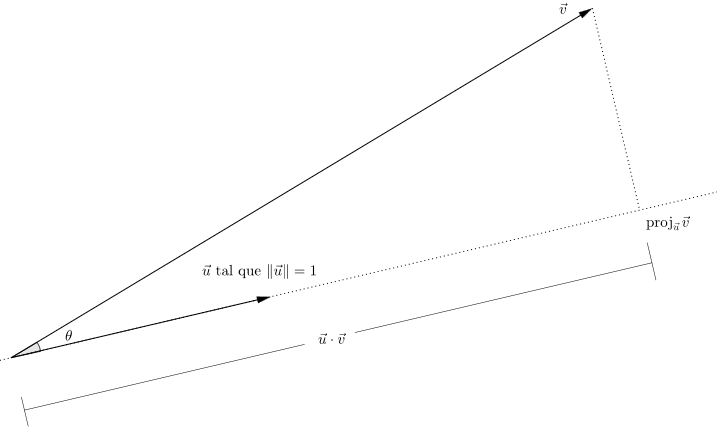
\includegraphics[width=1\linewidth]{\dir/Semana11/semana11-proj}
	\end{center}
\end{figure} Gostaríamos de encontrar a componente do vetor na direção da reta tracejada. Para isto, podemos considerar um vetor \textit{unitário} $\vec{u}$ sobre a reta. Assim, a componente de $\vec{v}$ na direção de $\vec{u}$ é igual a $k \vec{u}$, onde $k$ tem a ver com o cosseno do ângulo entre os vetores:
\begin{equation}
\cos \theta = \frac{\text{cateto adjacente}}{\text{hipotenusa}} = \frac{k}{\|\vec{v}\|}.
\end{equation} Utilizando novamente que $\vec{u}$ é um vetor unitário (isto é, $\|\vec{u}\|=1$), concluimos que
\begin{equation}
k = \|\vec{v}\| \cos \theta = \|\vec{u}\| \|\vec{v}\| \cos \theta = \vec{u} \cdot \vec{v}.
\end{equation} Assim sendo, definimos a \textbf{projeção ortogonal de $\vec{v}$ em um vetor unitário $\vec{u}$} como sendo
\begin{equation}
\boxed{\proj_{\vec{u}} \vec{v} = (\vec{u} \cdot \vec{v}) \, \vec{u}.}
\end{equation} No \textbf{caso onde $\vec{u}$ não está normalizado}, devemos primeiramente normalizar o vetor, de modo que a projeção ortogonal é dada por
\begin{equation}
\boxed{\proj_{\vec{u}} \vec{v} = \bigg( \frac{\vec{u}}{\|\vec{u}\|} \cdot \vec{v} \bigg) \, \frac{\vec{u}}{\|\vec{u}\|} = \frac{\vec{u} \cdot \vec{v}}{\|\vec{u}\|^2} \, \vec{u} = \frac{\vec{u} \cdot \vec{v}}{\vec{u} \cdot \vec{u}} \, \vec{u}.}
\end{equation}

\begin{example}\label{canon}
	Considere vetores no espaço de quatro dimensões $\mathbb{R}^4$. Vamos determinar a projeção do vetor $\vec{v} =
	\begin{bmatrix}
	1 \\ -1 \\ 3 \\ 4
	\end{bmatrix}$ na direção da reta que tem a mesma direção do vetor $\vec{u} =
	\begin{bmatrix}
	1 \\ 1 \\ 1 \\ -1
	\end{bmatrix}.$ Observamos inicialmente que $\|\vec{u}\| = \sqrt{4} = 2$ não é unitário. Temos que
	\begin{equation}
	\proj_{\vec{u}} \vec{v} =  \frac{\vec{u} \cdot \vec{v}}{\|\vec{u}\|^2} \, \vec{u} = \frac{1 - 1 + 3 - 4}{4}
	\begin{bmatrix}
	1 \\ 1 \\ 1 \\ -1
	\end{bmatrix} =
	-\frac{1}{4}
	\begin{bmatrix}
	1 \\ 1 \\ 1 \\ -1
	\end{bmatrix} =
	\begin{bmatrix}
	1/4 \\ 1/4 \\ 1/4 \\ -1/4
	\end{bmatrix}.
	\end{equation} A projeção de $\vec{v}$ sobre o vetor $\vec{e}_3$ da base canônica de $\mathbb{R}^4$ é (observe que $\|\vec{e}_3\| = 1$)
	\begin{equation}
	\proj_{\vec{e}_3} \vec{v} = (\vec{e}_3 \cdot \vec{v}) \, \vec{e}_3 = (0 + 0 + 3 + 0)
	\begin{bmatrix}
	0 \\ 0 \\ 1 \\ 0
	\end{bmatrix} = \begin{bmatrix}
	0 \\ 0 \\ 3 \\ 0
	\end{bmatrix}.
	\end{equation} Observe que a projeção sobre o vetor $\vec{e}_3$ da base canônica apenas ``enfatiza'' a terceira componente do vetor $\vec{v}$. Isto é bastante natural, pois $\vec{v} \cdot \vec{e}_3$ deve fornecer o comprimento da projeção de $\vec{v}$ na direção do vetor unitário $\vec{e}_3$, que deve ser igual a terceira componente do vetor. É justamente assim que usamos a base canônica para representar vetores geometricamente. De forma geral, podemos escrever
	\begin{equation}
	\vec{v} = \big( \vec{v} \cdot \vec{e}_1 \big) \vec{e}_1 + \big( \vec{v} \cdot \vec{e}_2 \big) \vec{e}_2  + \big( \vec{v} \cdot \vec{e}_3 \big) \vec{e}_3  + \big( \vec{v} \cdot \vec{e}_4 \big) \vec{e}_4.
	\end{equation} Este tipo de represetação será explorado com mais detalhes na próxima seção$. \ \lhd$
\end{example}

As projeções ortogonais também podem ser utilizadas para o cálculo de distâncias de ponto à retas que passam pela origem: Pela interpretação geométrica da subtração de vetores, obtemos um vetor perpendicular à reta com a direção de $\vec{u}$ e que termina onde termina o vetor $\vec{v}$ (ver figura).
\begin{figure}[h!]
	\begin{center}
		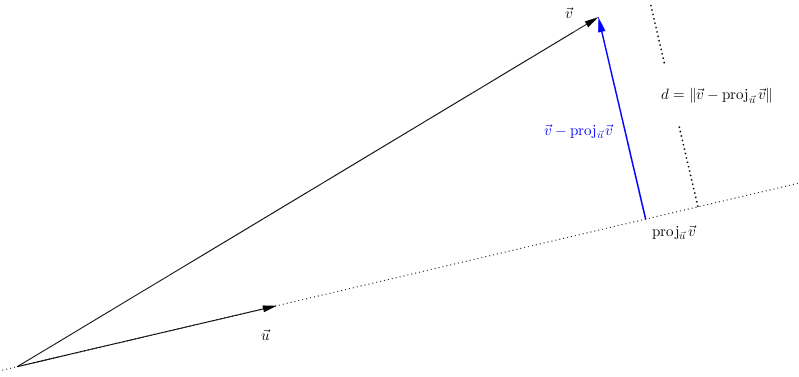
\includegraphics[width=1\linewidth]{\dir/Semana11/semana11-dist}
	\end{center}
\end{figure}

\noindent Desta maneira, o comprimento deste vetor, a saber $\|\vec{u} - \proj_{\vec{u}} \vec{v}\|$, é a distância procurada.\footnote{Lembre: a distância de um ponto a uma reta é a menor distância entre este ponto e os pontos da reta; por esta razão que procuramos um vetor perpendicular à reta.}

\begin{example}
	Calcular a distância do ponto $P = (0,2,3)$ e a reta que passa pela origem e tem a direção do vetor $\vec{u} =
	\begin{bmatrix}
	1 \\ 2 \\1
	\end{bmatrix}.$
	
	Para isto, consideramos o vetor $\vec{v}$ cujas componentes são as componentes do ponto $P$. Assim, estamos na situação da discussão acima e vale que
	\begin{equation}
	\proj_{\vec{u}} \vec{v} = \frac{7}{6}
	\begin{bmatrix}
	1 \\ 2 \\1
	\end{bmatrix} \implies
	\vec{u} - \proj_{\vec{u}} \vec{v} =
	\begin{bmatrix}
	0 \\ 2 \\ 3
	\end{bmatrix} - \frac{7}{6}
	\begin{bmatrix}
	1 \\ 2 \\1
	\end{bmatrix} =
	\begin{bmatrix}
	-7/6 \\ -1/3 \\ 11/6
	\end{bmatrix}.
	\end{equation} Portanto,
	\begin{equation}
	d = \|\vec{u} - \proj_{\vec{u}} \vec{v}\| = \frac{\sqrt{49 + 1 + 121}}{6} = \frac{\sqrt{171}}{6} \simeq 2,18.
	\end{equation}
\end{example}

\begin{exercise}
	Como poderíamos fazer se a reta não passasse pela origem? O mesmo raciocínio funciona?
\end{exercise}

\subsection*{Exercícios resolvidos}

\construirExeresol

\subsection*{Exercícios}

\construirExer

\section{Bases ortogonais e ortonormais}


Vimos que uma das importâncias do produto escalar é estender o conceito de ortogonalidade para espaços vetoriais mais gerais. A ortogonalidade traz consigo a noção de projeção ortogonal. Agora vamos ver algumas vantagens em se considerar bases de espaços vetoriais que são também conjuntos ortogonais; estas são conhecidas como \textbf{bases ortogonais}.

\begin{example}\label{ortonormal}
	A base canônica de $\mathbb{R}^n$ forma um conjunto ortogonal e é, portanto, uma base ortogonal. Assim como no Exemplo \ref{canon}, é possível representar qualquer vetor $\vec{v}$ como
	\begin{equation}
	\vec{v} = \big( \vec{v} \cdot \vec{e}_1 \big) \vec{e}_1 + \big( \vec{v} \cdot \vec{e}_2 \big) \vec{e}_2  + \cdots  + \big( \vec{v} \cdot \vec{e}_n \big) \vec{e}_n.
	\end{equation}
\end{example}

Vejamos que esta propriedade da base canônica é, na realidade, uma propriedade de todas as bases ortogonais:

\begin{theorem}\label{thm:base-ortogonal}
	Seja $\mathcal{B} = \{ \vec{v}_1, \vec{v}_2, \cdots, \vec{v}_n\}$ uma base ortogonal de $\mathbb{R}^n$. Então qualquer vetor $\vec{v} \in \mathbb{R}^n$ pode ser representado como
	\begin{equation}
	\vec{v} = \frac{\vec{v} \cdot \vec{v}_1}{\vec{v}_1 \cdot \vec{v}_1} \, \vec{v}_1 + \frac{\vec{v} \cdot \vec{v}_2}{\vec{v}_2 \cdot \vec{v}_2} \, \vec{v}_2  + \cdots  + \frac{\vec{v} \cdot \vec{v}_n}{\vec{v}_n \cdot \vec{v}_n} \, \vec{v}_n.
	\end{equation} Podemos escrever, de outra maneira, que
	\begin{equation}
	\vec{v} = \proj_{\vec{v}_1} \vec{v} +  \proj_{\vec{v}_2} \vec{v}  + \cdots  + \proj_{\vec{v}_n} \vec{v}.
	\end{equation}
\end{theorem}

Este resultado mostra que bases ortogonais são especiais e boas de trabalhar. Lembra que anteriormente, para encontrar os coeficientes de um vetor em uma base, tínhamos que encontrar $c_1, c_2, \cdots, c_n$ resolvendo o sistema linear cuja forma vetorial é
\begin{equation}
c_1 \vec{v}_1 + c_2 \vec{v}_2 + \cdots + c_n \vec{v}_n = \vec{v}.
\end{equation} O teorema acima afirma, em outras palavras, quando a base é ortogonal, os coeficientes do vetor $\vec{v}$ na base $\mathcal{B}$ são os números
\begin{equation}
c_j = \frac{\vec{v} \cdot \vec{v}_j}{\vec{v}_j \cdot \vec{v}_j}.
\end{equation}

\begin{proof}[Justificativa do Teorema \ref{thm:base-ortogonal}]
	Se a representação do vetor $\vec{v}$ na base $\mathcal{B}$ for
	\begin{equation}
	\vec{v} = c_1 \vec{v}_1 + c_2 \vec{v}_2 + \cdots + c_n \vec{v}_n,
	\end{equation} então, fazendo o produto escalar desta expressão com $\vec{v}_j$ e utilizando as propriedades de ortogonalidade, concluimos que
	\begin{equation}
	\vec{v} \cdot \vec{v}_j = \big( c_1 \vec{v}_1 + c_2 \vec{v}_2 + \cdots + c_n \vec{v}_n \big) \cdot \vec{v}_j = c_1 (\vec{v}_1\cdot \vec{v}_j) + c_2 (\vec{v}_2\cdot \vec{v}_j) + \cdots + c_n (\vec{v}_n\cdot \vec{v}_j) = c_j \big( \vec{v}_j \cdot \vec{v}_j \big),
	\end{equation} pois $\vec{v}_i \cdot \vec{v}_j = 0$ sempre que $i \neq j$. Daí, concluimos, como queríamos, que os coeficientes devem satisfazer
	\begin{equation}
	c_j = \frac{\vec{v} \cdot \vec{v}_j}{\vec{v}_j \cdot \vec{v}_j}. \qedhere
	\end{equation}
\end{proof}

\begin{example}
	Vamos justificar que os vetores
	\begin{equation}
	\vec{u} =
	\begin{bmatrix}
	4 \\ 2
	\end{bmatrix} \ \ \text{ e }\ \
	\vec{v} =
	\begin{bmatrix}
	-1 \\ 2
	\end{bmatrix}
	\end{equation} formam uma base ortogonal para $\mathbb{R}^2$.
	
	Em primeiro lugar, formam uma base, pois são vetores linearmente independentes e são dois (que é a dimensão de $\mathbb{R}^2$). Agora, calculamos
	\begin{equation}
	\vec{u} \cdot \vec{v} = 4\cdot (-1) + 2\cdot 2 = 0.
	\end{equation} Segue que $\vec{u}$ e $\vec{v}$ são também ortogonais e, logo, formam uma base ortogonal de $\mathbb{R}^2$.
	
	Para escrever um vetor $\vec{x} =
	\begin{bmatrix}
	2 \\ -7
	\end{bmatrix}$ nesta base, podemos calcular as projeções nos elementos da base (isto apenas vale se os elementos da base são ortogonais!):
	\begin{equation}
	\vec{x} = \frac{\vec{x} \cdot \vec{u}}{\vec{u} \cdot \vec{u}} \, \vec{u} + \frac{\vec{x} \cdot \vec{v}}{\vec{v} \cdot \vec{v}} \, \vec{v} = \frac{-6}{20} \, \vec{u} + \frac{-16}{5} \, \vec{v} = -0.3 \, \vec{u} -3.2 \, \vec{v}. \ \lhd
	\end{equation}
\end{example}


Observe no exemplo acima que é muito mais fácil obter as componentes por ortogonalidade do que resolver sistemas lineares. Isto mesmo em dimensão baixa! Imagine se fosse um sistema $5\times 5$ ou ainda maior.


Note que a base canônica, como no Exemplo \ref{ortonormal}, tem a propriedade adicional que $\|\vec{e}_j\| = 1$ para todo índice $j$. Isto fez com que a representação de vetores do Teorema \ref{thm:base-ortogonal} assumisse um formato ainda mais simples. Estas bases ortogonais que tem por elementos vetores unitários são conhecidas como \textbf{bases ortonormais}. Mais explicitamente, uma base ortonormal é uma base $\{\vec{v}_1, \vec{v}_2, \cdots, \vec{v}_n\}$ de um espaço vetorial que adicionalmente satisfaz
\begin{equation}
\vec{v}_i \cdot \vec{v}_j = 0 \text{ para } i \neq j \text{ e também } \|\vec{v}_j\| = 1 \text{ para todo } j \ \ \big( \iff \vec{v}_j \cdot \vec{v}_j = 1 \big)
\end{equation} Uma consequência imediata é que, sendo $\{\vec{v}_1, \vec{v}_2, \cdots, \vec{v}_n\}$ uma base ortonormal de $\mathbb{R}^n$, podemos escrever
\begin{equation}
\vec{v} = \big( \vec{v} \cdot \vec{v}_1 \big) \vec{v}_1 + \big( \vec{v} \cdot \vec{v}_2 \big) \vec{v}_2  + \cdots + \big( \vec{v} \cdot \vec{v}_n \big) \vec{v}_n.
\end{equation}

\begin{example}
	Os vetores
	\begin{equation}
	\vec{u} =
	\begin{bmatrix}
	1 \\ 0 \\ 0
	\end{bmatrix}, \
	\vec{v} =
	\begin{bmatrix}
	0 \\ \sqrt{2}/2 \\ \sqrt{2}/2
	\end{bmatrix}, \ \text{e }
	\vec{w} =
	\begin{bmatrix}
	0 \\ \sqrt{2}/2 \\ - \sqrt{2}/2
	\end{bmatrix}
	\end{equation} formam uma base ortonormal de $\mathbb{R}^3$: verifique! Qualquer vetor $\vec{x} \in \mathbb{R}^3$ pode ser escrito como 
	\begin{equation}
	\vec{x} = \big( \vec{x} \cdot \vec{u} \big) \vec{u} + \big( \vec{x} \cdot \vec{v} \big) \vec{v} + \big( \vec{x} \cdot \vec{w} \big) \vec{w}
	\end{equation} Por exemplo,
	\begin{equation}
	\vec{x} =
	\begin{bmatrix}
	2 \\ -1 \\ 1
	\end{bmatrix} = 2 \vec{u} + 0 \vec{v} - \sqrt{2} \vec{w} = 2 
	\begin{bmatrix}
	1 \\ 0 \\ 0
	\end{bmatrix} + \sqrt{2} 
	\begin{bmatrix}
	0 \\ \sqrt{2}/2 \\ - \sqrt{2}/2
	\end{bmatrix}.
	\end{equation}
\end{example}


Observamos finalmente que bases ortogonais podem ser facilmente transformadas em bases ortonormais pelo processo de normalização.


\begin{example}
	Os vetores 
	\begin{equation}
	\vec{u} =
	\begin{bmatrix}
	1 \\ 1 \\ 1
	\end{bmatrix}, \
	\vec{v} =
	\begin{bmatrix}
	1 \\ 0 \\ -1
	\end{bmatrix} \ \text{e }
	\vec{w} =
	\begin{bmatrix}
	1 \\ -2 \\ 1
	\end{bmatrix}
	\end{equation} formam uma base ortogonal de $\mathbb{R}^3$. Normalizando cada um dos vetores, podemos obter uma base ortonormal de $\mathbb{R}^3$:
	\begin{equation}
	\left\{
	\begin{array}{ll}
	\|\vec{u}\| = \sqrt{1 + 1 + 1} = \sqrt{3} \\
	\|\vec{v}\| = \sqrt{1 + 1} = \sqrt{2} \\
	\|\vec{w}\| = \sqrt{1 + 4 + 1} = \sqrt{6} \\
	\end{array}
	\right.
	\end{equation} Isto implica que os vetores
	\begin{equation}
	\frac{\vec{u}}{\|\vec{u}\|} = \frac{1}{\sqrt{3}}
	\begin{bmatrix}
	1 \\ 1 \\ 1
	\end{bmatrix} = 
	\begin{bmatrix}
	1/\sqrt{3} \\ 1/\sqrt{3} \\ 1/\sqrt{3}
	\end{bmatrix}, \
	\frac{\vec{v}}{\|\vec{v}\|} = \frac{1}{\sqrt{2}}
	\begin{bmatrix}
	1 \\ 0 \\ -1
	\end{bmatrix} =
	\begin{bmatrix}
	1/\sqrt{2} \\ 0 \\ -1/\sqrt{2}
	\end{bmatrix} \ \text{e }
	\frac{\vec{w}}{\|\vec{w}\|} = \frac{1}{\sqrt{6}}
	\begin{bmatrix}
	1 \\ -2 \\ 1
	\end{bmatrix} = 
	\begin{bmatrix}
	1/\sqrt{6} \\ -2/\sqrt{6} \\ 1/\sqrt{6}
	\end{bmatrix}
	\end{equation} formam um base ortonormal de $\mathbb{R}^3. \ \lhd$
\end{example}

\subsection*{Exercícios resolvidos}

\construirExeresol

\subsection*{Exercícios}

\construirExer

\section{Exercícios finais}

\construirExer

\end{document} 
